% Copyright (c) 2008-2009 solvethis
% Copyright (c) 2010-2016,2018-2019,2021 Casper Ti. Vector
% Copyright (c) 2021 Kurapica
% Copyright (c) 2021 iofu728
% Overleaf version.

%*********************************************************************
% iofu728-pkuthss: 北京大学研究生学位论文模板
% 2021/06/09 v1.0.0
%
% 重要提示:
%   1. 当前overleaf版符合2021研究生学位论文要求,可通过图书馆审核
%   2. 当前版本基于pkuthss v1.9.0
%   3. 请使用UTF-8编码,XeLaTeX方式编译
%   4. 请仔细阅读用户文档
%   5. 修改、使用、发布本文档类请务必遵循LaTeX Project Public License和知识共享4.0
%   6. 如有疑问github/iofu728/pkuthss上提问或联系作者@iofu728
%*********************************************************************

\documentclass[fontset=fandol,ugly]{pkuthss}
  % 学位论文模式  ugly    (默认打开,请保留)
  % 盲审模式      blind   (默认关闭)
  % 字体库        fontset
  %   auto | windows | windows@overleaf | mac | fandol | ubuntu | none
  % windows*, mac为商业字体,如需使用请遵循相应版权协议(默认下overleaf中不可用)
  % fandol与windows效果相近,但字符库偏少,推荐使用(默认);
  % ubuntu字体效果偏差较大; 设为none时需自行配置字体集;

\usepackage[backend=biber,style=gb7714-2015]{biblatex}
  % 参考文献遵循GB/T 7714-2015标准,使用biblatex-gb7714-2015 宏包。
  % 此处使用顺序编码制,如使用著者-出版年制则更改为b7714-2015ay。

% 示例文档用包和设定,该段均可移除.
\usepackage{enumitem,fancyvrb}
\usepackage{booktabs,multirow,longtable,makecell} % 表格相关
\RecustomVerbatimEnvironment{Verbatim}{Verbatim}{frame = single, tabsize = 4, fontsize=\footnotesize}
\renewcommand{\v}[1]{\boldsymbol{#1}}
\newcommand\pkg[1]{\textsf{#1}}

% 参考文献边距字体
\setlength{\bibitemsep}{3bp}
\renewcommand*{\bibfont}{\zihao{5}\linespread{1.27}\selectfont}

\pkuthssinfo{
	cthesisname = {数字图像处理期末作業},
 	thesiscover = {数字图像处理期末作業},
	ethesisname = {Homework},
	ctitle = {面向网路教学的听课状态视频分析系统},
	etitle = {Homework},
	%cauthor = {干皓丞}, 
	eauthor = {Kan, Hao-Cheng},
	%studentid = {2101212850},
	teamname = {易思达、郑翰浓、\\徐华阳、 干皓丞},
	% 具体时间以教务为准,初稿3月,送审4月,答辩5月,最终6月。
	%date = {\zhdigits{2021}\ \ 年\ \ \zhnumber{6}\ \ 月},
	date = {\zhdigits{2022}\ \ 年\ \ \zhnumber{5}\ \ 月},
	school = {信息工程学院},
	cmajor = {计算机应用技术}, emajor = {通信及信息安全技术},
	direction = {通信及信息安全技术},
	%mentorlines = {2}, % 导师个数
	mentorlines = {1}, % 导师个数
	% 副教授 A.P. 讲师 Lec.
	cmentor = {刘宏\ \ 教授}, ementor = {Prof.\ XXX },
	%cmentor = {XXX\ \ 教授\\YYY\ \ 教授}, ementor = {Prof.\ XXX and Prof.\ YYY},
	ckeywords = {可用教育系统},
	ekeywords = {A,B,C,D},
	% 盲审模式参数, 需在documentclass增加blind
	blindid = {XXXXXXXXX}, discipline = {XXXX}
}
\addbibresource{ref.bib}

\begin{document}
	\frontmatter
	\pagestyle{empty}
	\maketitle
	\cleardoublepage
	% 需替换门户版权声明pdf
	%% Copyright (c) 2008-2009 solvethis
% Copyright (c) 2010-2017,2021 Casper Ti. Vector
% Copyright (c) 2021 iofu728
% All rights reserved.
%
% Redistribution and use in source and binary forms, with or without
% modification, are permitted provided that the following conditions are
% met:
%
% * Redistributions of source code must retain the above copyright notice,
%   this list of conditions and the following disclaimer.
% * Redistributions in binary form must reproduce the above copyright
%   notice, this list of conditions and the following disclaimer in the
%   documentation and/or other materials provided with the distribution.
% * Neither the name of Peking University nor the names of its contributors
%   may be used to endorse or promote products derived from this software
%   without specific prior written permission.
%
% THIS SOFTWARE IS PROVIDED BY THE COPYRIGHT HOLDERS AND CONTRIBUTORS "AS
% IS" AND ANY EXPRESS OR IMPLIED WARRANTIES, INCLUDING, BUT NOT LIMITED TO,
% THE IMPLIED WARRANTIES OF MERCHANTABILITY AND FITNESS FOR A PARTICULAR
% PURPOSE ARE DISCLAIMED. IN NO EVENT SHALL THE COPYRIGHT HOLDER OR
% CONTRIBUTORS BE LIABLE FOR ANY DIRECT, INDIRECT, INCIDENTAL, SPECIAL,
% EXEMPLARY, OR CONSEQUENTIAL DAMAGES (INCLUDING, BUT NOT LIMITED TO,
% PROCUREMENT OF SUBSTITUTE GOODS OR SERVICES; LOSS OF USE, DATA, OR
% PROFITS; OR BUSINESS INTERRUPTION) HOWEVER CAUSED AND ON ANY THEORY OF
% LIABILITY, WHETHER IN CONTRACT, STRICT LIABILITY, OR TORT (INCLUDING
% NEGLIGENCE OR OTHERWISE) ARISING IN ANY WAY OUT OF THE USE OF THIS
% SOFTWARE, EVEN IF ADVISED OF THE POSSIBILITY OF SUCH DAMAGE.

% 此处不用 \specialchap,因为学校要求目录不包括其自己及其之前的内容。
\chapter*{版权声明}
% 综合学校的书面要求及 Word 模版来看,版权声明页不用加页眉、页脚。
\thispagestyle{empty}

任何收存和保管本论文各种版本的单位和个人,
未经本论文作者同意,不得将本论文转借他人,
亦不得随意复制、抄录、拍照或以任何方式传播。
否则一旦引起有碍作者著作权之问题,将可能承担法律责任。

% 替换门户下载pdf
\begin{textblock}{1}(-0.8,-0.08)
    \colorbox{white}{
        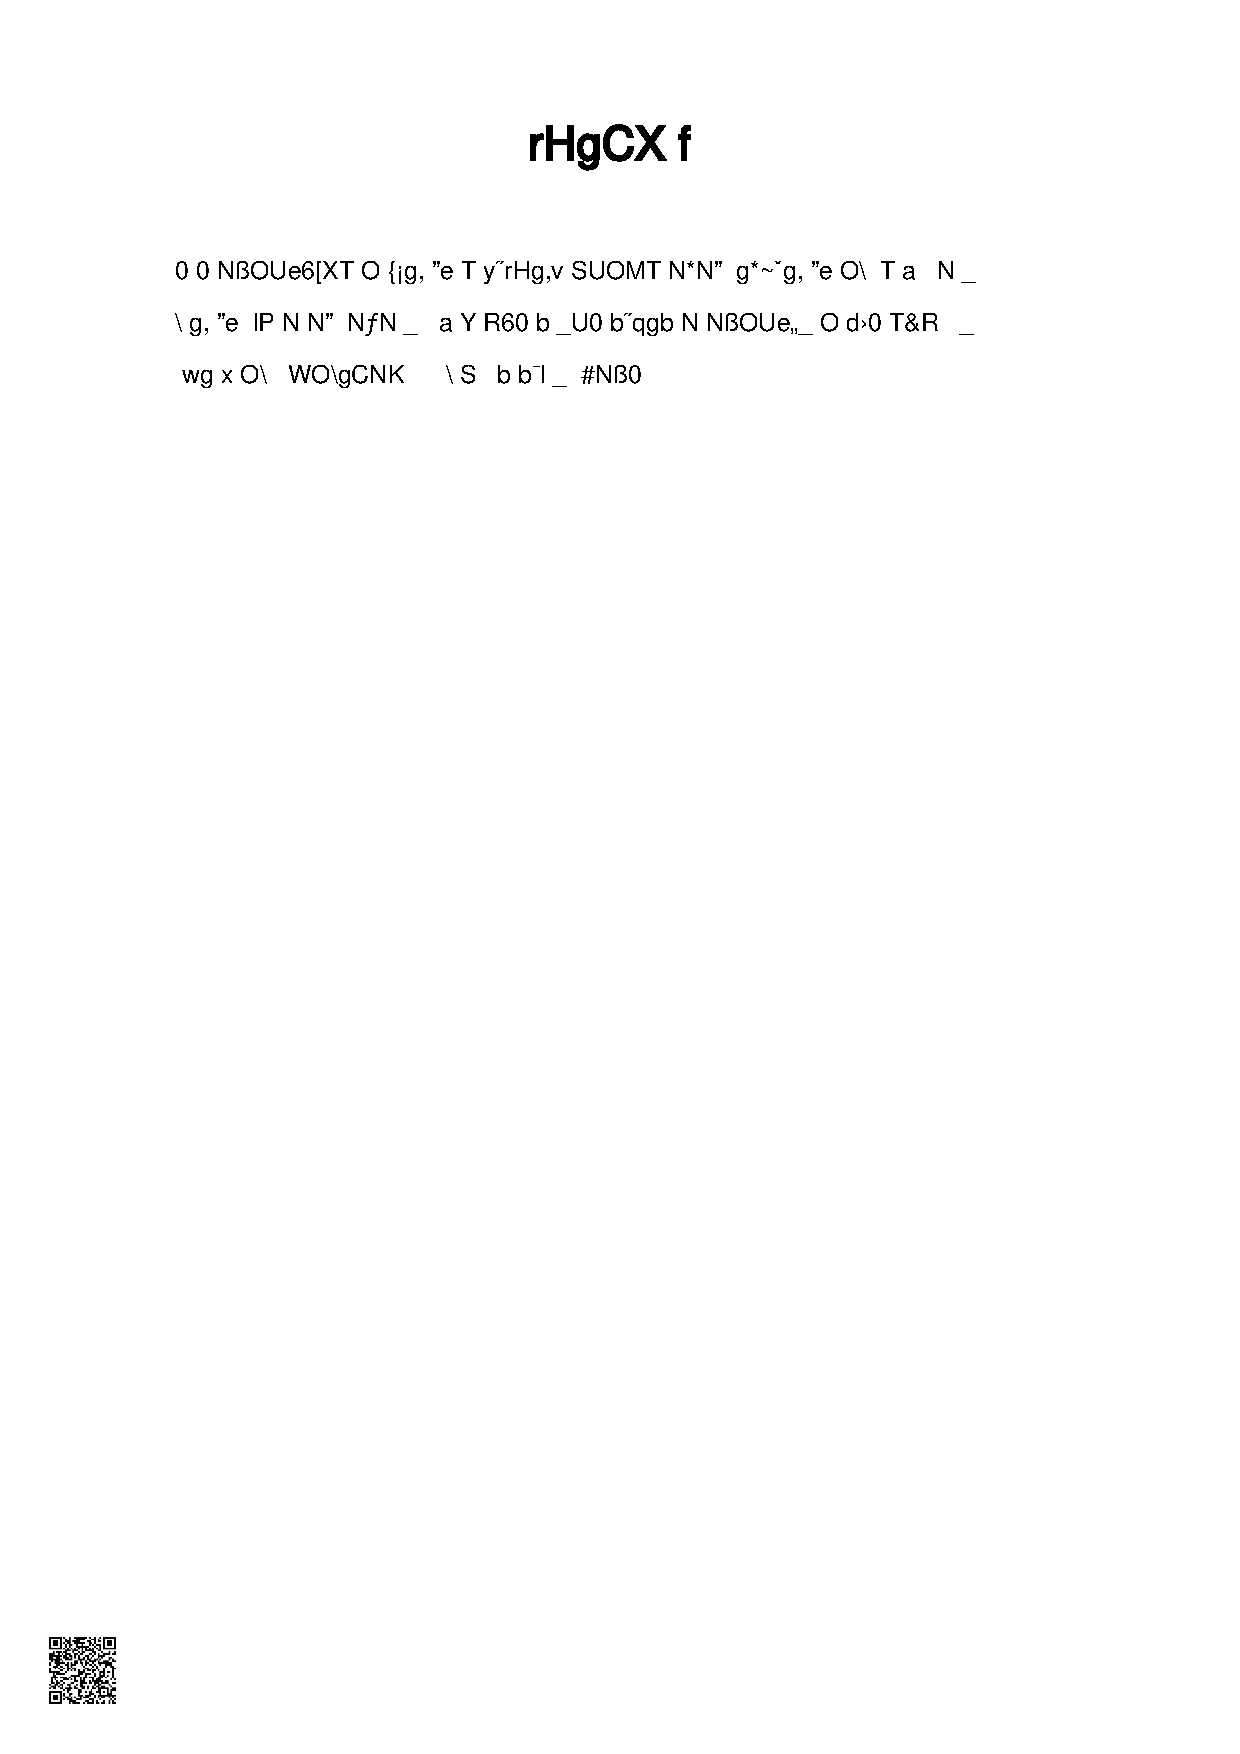
\includegraphics[height = 1.2448\textheight]{img/bqsm_180xxxxxxx.pdf}
    }
\end{textblock}

% vim:ts=4:sw=4

	\cleardoublepage
	\pagestyle{plain}
	\setcounter{page}{0}
	\pagenumbering{Roman}
	\begin{cabstract}

本次数字图像处理期末作业,为尝试建立一个面向网路教学的听课状态视频分析系统,在过程中对可能会用到的目前主流的前端框架与后端框架前沿技术进行调研,随后进行测试,同时也为了开发流程尝试不同技术跟工具。也对听课状态视频分析系统进行可行性分析与系统规划。

本次作业相关专案于 GitHub:

https://github.com/kancheng/2022-dip-final-report-for-deeplearning-system

\begin{figure}[htb]
\centering 

\includegraphics[width=0.30\textwidth]{img/dip-final-qr.png} 
\caption{kancheng/2022-dip-final-report-for-deeplearning-system}
\label{Test}
\end{figure}



\end{cabstract}

%\begin{eabstract}
%    英文摘要部分...
%\end{eabstract}

% vim:ts=4:sw=4

	\tableofcontents
	% 如有需要使用主要符号对照表
	\begin{denotation}

\item[$x,y,m,n,t$] 标量,通常为变量
\item[$K,L,D,M,N,T$] 标量,通常为超参数
\item[$x\in \mathbb{R}^{D}$] D维列向量
\item[$(x_1,\cdots,x_D)$] D维行向量
\item[$(x_1,\cdots,x_D)^T$ or $(x_1;\cdots;x_D)^T$]  D维行向量
\item[$x\in \mathbb{R}^{KD}$]  ($KD$)维的向量
\item[$\mathbb{M}_i$ or $\mathbb{M}_i(\v x)$]  第$i$列为$\v 1$(或者$\v x$),其余为$\v 0$的矩阵
\item[$diag(\v x)$]  对角矩阵,其对角元素为$\v x$
\item[$\v I_N$ or $I$]  ($N\times N$)的单位阵
\item[$\v A \in \mathbb{R}^{D_1\times D_2\times \cdots \times D_K}$]  大小为$D_1\times D_2\times \cdots \times D_K$的张量
\item[$\{x^{(n)}\}^{N}_{n=1}$]  集合
\item[$\{(x^{(n)},y^{(n)})\}^{N}_{n=1}$]  数据集
\item[$\mathcal{N}(\v x;\mu,\sum)$]  变量$x$服从均值为$\mu$,方差为$\sum$的高斯分布

\end{denotation}

\footnotetext[1]{本符号对照表内容选自\citeauthor{qiu2020nndl}老师的《神经网络与深度学习》\cite{qiu2020nndl}一书。}


	\mainmatter
	\chapter{系统分析与规划}
\label{chap:1}

此节目标是为了建立一个面向网路教学的听课状态视频分析系统,该章节讨论该系统的目标架构,并说明实际完成的部分。此章节也会针对初期可运用的技术逐一进行说明。

\section{系统规划}

由于本作业将面向网路教学的听课状态视频分析系统,在作为实际的产品进行规划,实际需要的功能分为九个项目,其项目为会员功能、视频观看、作业缴交、教学直播、学习检测、代码提交、签到功能、课堂抢答、考试功能。

\subsection{功能概念规划}

\begin{figure}[htb]
\centering 
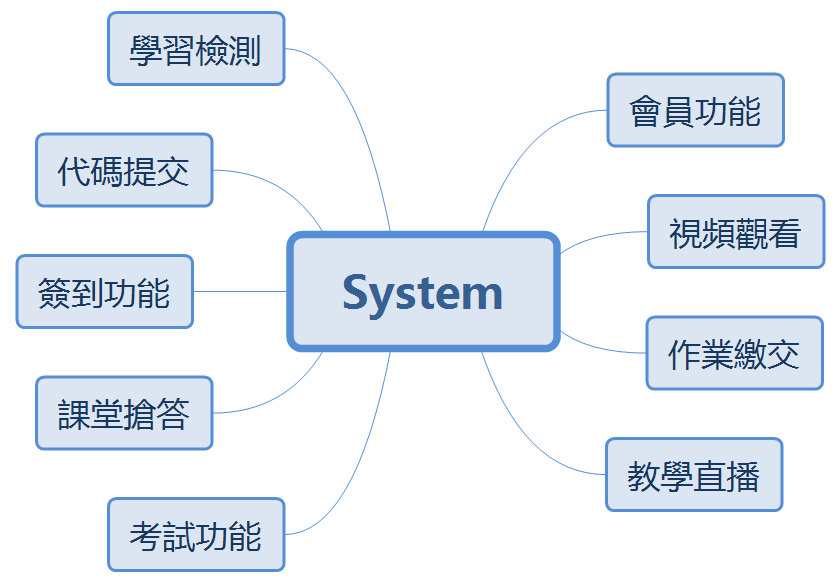
\includegraphics[width=0.60\textwidth]{img/ch1m1.png} 
\caption{系统功能面规划}
\label{Test}
\end{figure}

\begin{itemize}
\item [-] 会员功能 : 其会员系统分为老师使用者、学生使用者、系统管理者。
\item [-] 视频观看 : 为播放上课视频录影或者是老师预先上传的教学录影视频。
\item [-] 作业缴交 : 为作业缴交功能。
\item [-] 教学直播 : 为针对教学现场的直播,该功能与考试功能、课堂抢答、学习检测相关。
\item [-] 学习检测 : 为协助老师判断学生精神状况的功能。老师在教学直播或者视频观看两大功能中,可设定对学生当下的学习状况进行判断的请求,当学生同意后,系统则会搜集学生执行系统的电脑镜头,并对镜头前的状况进行疲劳或者注意力的判断。最后产生统计报表。
\item [-] 代码提交 : 为类似 GitHub 的版本控制,学生提交代码作业后,该系统除了收纳外,过程中会进行代码比对,可判断有无相互抄袭代码。
\item [-] 签到功能 : 与教学直播相关的连动功能。
\item [-] 课堂抢答 : 与教学直播相关的连动功能。
\item [-] 考试功能 : 分为大考与临时考试两种,由老师进行设定。
\end{itemize}

\subsection{功能概念关联}

该节说明各功能之间的关联,其使用者登入会员系统后,会根据使用者不同的权限而有不同的服务。当中课堂抢答、签到功能、学习检测都是要在使用者进入由老师方或者系统管理方使用者所发起的教学直播,才会接触到。当中学习检测功能则是不论视频观看或者教学直播功能中都能够发起。

\begin{figure}[htb]
\centering 
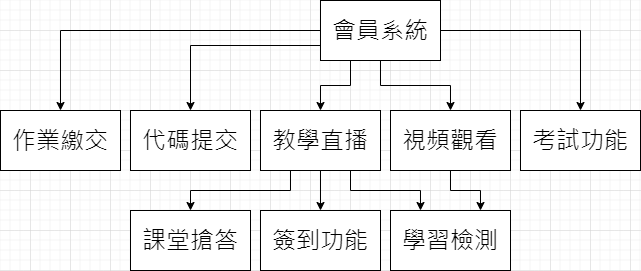
\includegraphics[width=0.80\textwidth]{img/ch1m2.png} 
\caption{关联说明}
\label{Test}
\end{figure}

\subsection{系统架构说明}

本系统架构分别为三大部分,一个是资料库,前端框架则是为 Vue,后端框架则是运用 Python Flask 作为主体的服务提供,而 Go 则是预计处理负责版本控制功能的部分。同时因为需要深度学习在计算机视觉的功能,在此会考量运用 Python 中的 Pytorch 或者是 Python 的 TensorFlow,这也是本作业考量使用 Python 作为主体开发方案的原因。

\begin{figure}[htb]
\centering 
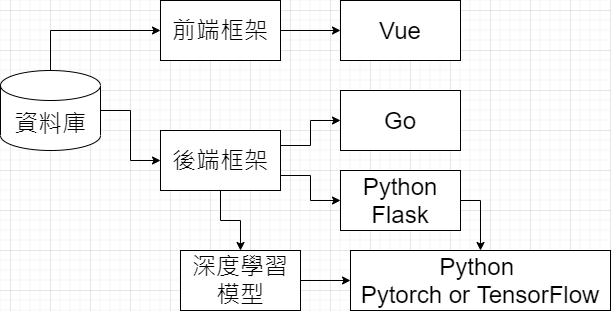
\includegraphics[width=0.80\textwidth]{img/ch1m3.png} 
\caption{关联说明}
\label{Test}
\end{figure}

\section{系统介面規劃}

此节为说明在系统规划中各个功能的预计线框图(Wireframe)的概念设计,其项目为会员功能、视频观看、作业缴交、教学直播、学习检测、代码提交、签到功能、课堂抢答、考试功能。

\subsection{会员功能}

在此会员功能分成三大部分,当中权限分为管理者、老师、学生三种权限,管理者拥有管理老师跟学生帐号的管理权限,同时也能够如老师帐号一样进行课堂直播与建立视频的课程,而老师帐号则是可以管理学生进入课堂,并且发起教学与进行课堂直播与建立视频的课程,同时可以询问学生进行学习效果的判断。

\begin{figure}[htb]
\centering 

\includegraphics[width=0.80\textwidth]{img/ch1m4.png} 
\caption{会员功能线框图}
\label{Test}
\end{figure}

\subsection{视频观看}

所谓的是频观看则分为两方描述,从学生角度来看,可以从老师上传的视频进入后进行观看,同时有一个笔记的按钮,该按钮的介面设计是可以开启一个支援 LaTeX 的编辑器,同时有着撷取老师录影画面,进行简易绘图笔记的功能,而笔记功能则是每个权限都可以使用。

另外还有一个课堂影片条列的功能,但由于老师跟管理员权限与学生不一致的缘故,故只有学生的画面中并没有增设学习状况判断的按钮。而从老师与管理员权限的角度来看,若在影片列表中设定增设学习状况的判断,那从学生的页面中则会看到,系统会跳出是否要让老师能够产生学习状况判断的讯息,若学生勾选否,则系统会在整班的报告中,回报该学生没有选同意此选项,而若学生选择同意,则系统会在整堂课随机时间利用使用者的摄像头,随机固定间隔时间拍照进行分析,行分析,产生出使用者目前学习的精神状况与判断,并将数据纪录下来进行统计并产生报表。

\begin{figure}[htb]
\centering 
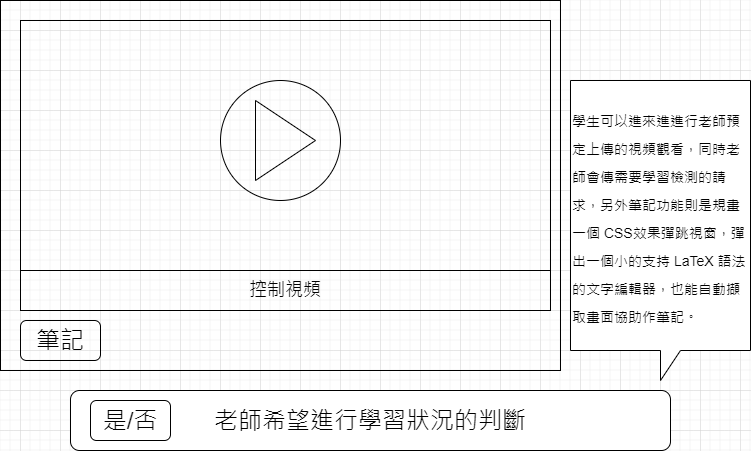
\includegraphics[width=0.80\textwidth]{img/ch1m5.png} 
\caption{视频观看页面的概念线框图}
\label{Test}
\end{figure}

\begin{figure}[htb]
\centering 
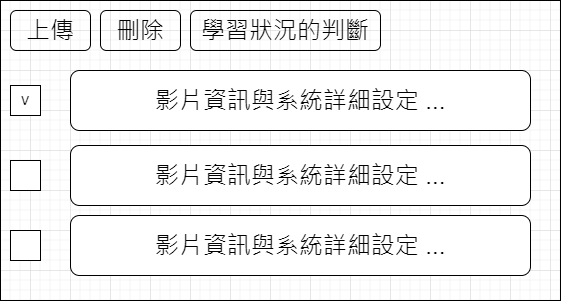
\includegraphics[width=0.50\textwidth]{img/ch1m6.png} 
\caption{视频观看的列表概念线框图}
\label{Test}
\end{figure}

\subsection{代码提交}

此节功能的现有方案为 gogs ,一个由开源社群开发的类似 GitHub 的项目代码管理平台,该方案由 Go 语言实现,若出于实际需求可能需要写整合的代码。但在此还是将其需求进行分析。从列表分析的页面为从管理员权限与老师的权限可用,此权限可以用代码交叉对比的功能,来判断学生间的代码是否互相抄袭,其功能实现则根据现有的开源套件进行整合,同时管理方与老师方也可以加入搜集来的范例去进行比对,如此一来类似助教可以在网路上爬取相关代码。一旦判断相似度高,则系统会给学生建议,请学生对其作业加入引用或者注明来源,鼓励学生除了自学之外,从其他资源的代码中学习到编程能力经验好的代码。另外代码提交页面,其功能类似于 GitHub 等开源项目管理平台的页面,当中可以提交程式码,并对其项目进行管理与版本控制,方便教授跟助教对学生的程式码进行批改。同时此部分支持学生团队开发协作,从而学习到对团队协作的软件开发工程经验。

\begin{figure}[htb]
\centering 
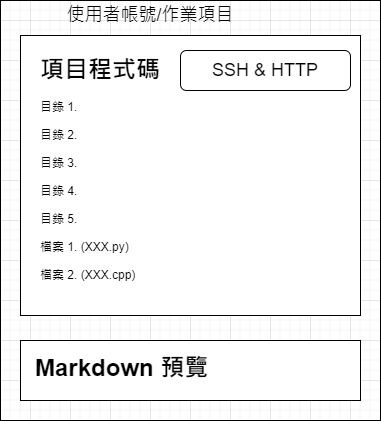
\includegraphics[width=0.40\textwidth]{img/ch1m8.png} 
\caption{代码提交的页面概念线框图}
\label{Test}
\end{figure}
\begin{figure}[htb]
\centering 
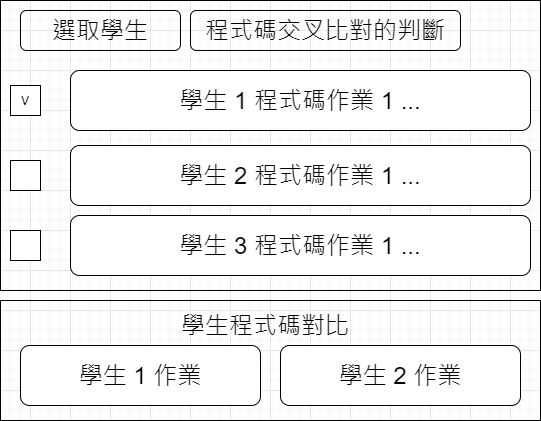
\includegraphics[width=0.50\textwidth]{img/ch1m7.png} 
\caption{代码提交列表的概念线框图}
\label{Test}
\end{figure}

\subsection{作业缴交}

在此现有整合的开源方案其中为 HackMD,同时该方案也有服务,为重要的笔记 Markdown 软体,但需求包含了 PDF、 Word、 Markdown、LaTeX 等档案类型,其复杂程度高,故尽可能使用现有的开源项目进行整合。而作业缴交页面的概念源自于学生权限的页面,由老师或者管理员权限建立课程发起作业后,学生提交相关档案,同时学生能够检视自己上传上来的文件。并且上传上来的文件可以进行档案版本的分类,从而协助管理档案的版本。

另外从列表的部分来看,该页概念为老师与管理权限可以运用文件内容交叉对比进行查核,若有相似性,则系统提供提醒,鼓励学生权限的使用者,引用与注明作业跟文献内容的来源。

\begin{figure}[htb]
\centering 
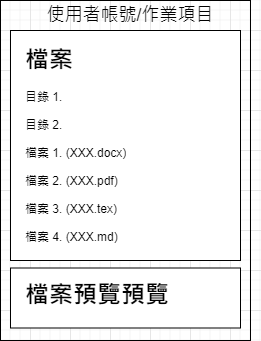
\includegraphics[width=0.50\textwidth]{img/ch1m9.png} 
\caption{作业缴交的页面概念线框图}
\label{Test}
\end{figure}

\begin{figure}[htb]
\centering 
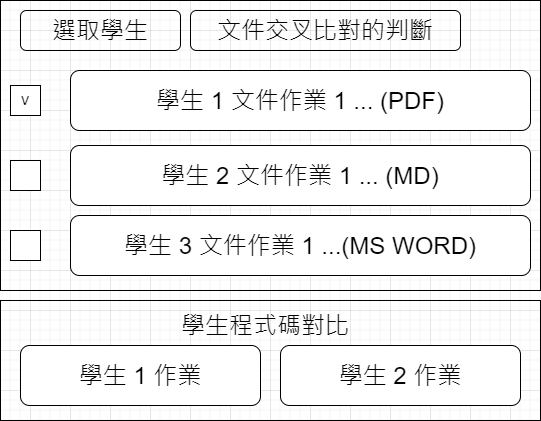
\includegraphics[width=0.80\textwidth]{img/ch1m10.png} 
\caption{作业缴交列表的概念线框图}
\label{Test}
\end{figure}


\subsection{教学直播}

此部分功能从老师与管理方来看,老师可以发起点名、抢答与学习状况的判断,而学生部分的则是可以回应,并且当中对过程的次数会进行纪录,同时发起抢答时,老师与管理方能设定秒数,此秒数会显示在学生方的按钮上,该秒数会倒数的状态,另外发起点名这个则是会累积,若学生方较晚才回应,老师的后台可以看到学生方在哪几次的点名于何时回应,而回应当下的时间则会于发起的点名时间互减,用来告知老师与管理方,学生点名的时间差。

另外与视频观看相同的地方在于,老师与管理端在此也能进行学习检测的功能发起,发起的当下,系统会提醒学生,并等待学生回应,若学生同意则运用该电脑的摄影机去随机抓出特定帧进行模型的判断,同时学生会在画面的另看到一角看到自己被判断的画面,最后该数据会统计,并回传给老师进行检视。

\begin{figure}[htb]
\centering 

\includegraphics[width=0.80\textwidth]{img/ch1m11.png} 
\caption{学生教学直播的页面概念线框图}
\label{Test}
\end{figure}

\begin{figure}[htb]
\centering 

\includegraphics[width=0.80\textwidth]{img/ch1m12.png} 
\caption{老师教学直播的页面概念线框图}
\label{Test}
\end{figure}


\subsection{学习检测}

学习检测功能是此次作业的重点,此部分有可能要拆成两部分来做,但在技术上很可能要用三个部分来看,第一个为前端画面 Vue、第二个为后段的 Flask、第三部分为 PyTorch 或者 TensorFlow 的深度学习模型整合,而从技术领域上,开发过程很可能要面对视频的处理,另外还有视频辨识所产生出来的分析,同时最后要生成老师方或者管理方可以分析的学习状态报表。同时判断学生是否在稳定的状态中进行学习也是很重要的一部分,此部分判断与规划的分析留待后面章节继续说明。

由下图可以知道,上图为可以判断的流程影像处理,当中原影像是随机从每一帧选取,其一是判断画面有没有人,其二判断有无可辨识的人脸,其三判断人眼的眼睛是否疲劳,其四则是判断人的表情是否疲惫。

\begin{figure}[htb]
\centering 

\includegraphics[width=0.80\textwidth]{img/ch1m13.png} 
\caption{学习检测页面概念线框图}
\label{Test}
\end{figure}

\subsection{考试功能}

考试功能为老师与管理方权限可以进行发起考试,当中考试可设为随堂考或者期末考,考题可以根据 CSV 、JSON、MS EXCEL 等不同格式来输入成为选择题,又或者是进入设定显示老师的问答题目。

\begin{figure}[htb]
\centering 
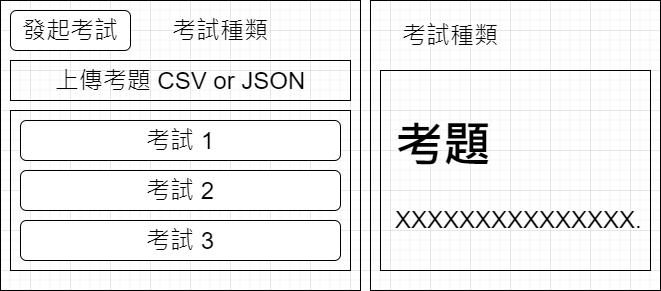
\includegraphics[width=0.80\textwidth]{img/ch1m14.png} 
\caption{考试功能页面概念线框图}
\label{Test}
\end{figure}

%\section{系统分析}
%\section{系统概念}
%\subsubsection{SSS1}

%\begin{itemize}
%\item [-][7,7] 空间卷积到 1*1*2048 然后一维卷积到 1*1*128
%\item [-]池化层到 1*1*2048 然后一维卷积到 1*1*128
%\end{itemize}


%\begin{itemize}
%\item Calculus
%\item Linear Algebra
%\item Basic Computer Concepts
%\end{itemize}

%\begin{description}
% \item[First] \hfill \\
% The first item
% \item[Second] \hfill \\
% The second item
% \item[Third] \hfill \\
% The third etc \ldots
%\end{description}

	\chapter{系统实现说明}
\label{chap:2}

本章重点在于说明运用技术的调研与说明目前主流可用方案,同时讲述系统规划。

\section{系统开发平台考量}

本作业在规划时考虑过在不同平台与不同方式开发的可行性方案,在应用程式开发上,若选择桌面开发可以使用 PyQt,而对应的行动装置上则可使用 React Native 使用 JS 技术开发完后,转成行动装置的 APP。

而使用网页技术开发,则考量可以运用 Web 的前后端开发,先完成桌面的应用跟规划后,再根据响应式网页的方式,将原有的桌面功能转为行动端的功能。而在此使用 Python Flask 与前端框架。

\begin{figure}[htb]
\centering 
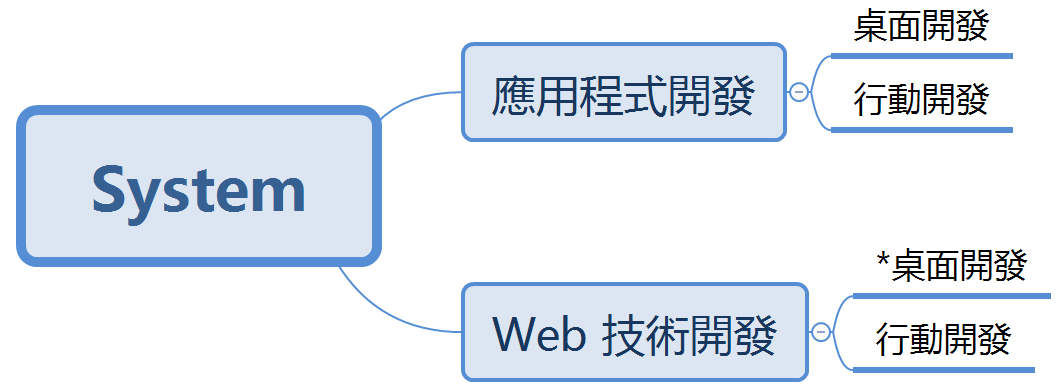
\includegraphics[width=0.80\textwidth]{img/ch2m0.png} 
\caption{系统开发方案}
\label{Test}
\end{figure}


%\begin{itemize}
%\item [-] L1
%\end{itemize}

\section{技术调研}

此节将本次作业所考量的技术与方案逐一进行说明,當中包含了前端框架、后端方案、应用程式方案與深度学习框架。

\subsection{前端框架}

在此作业中考量过三大前端的主流框架,分别是 Vue、Google 主导的 Angualr 框架与 脸书主导的 React 框架,根据开发的容易程度与开发团队的适应性,本作业最终选择了 Vue。其 Vue 的开发者尤雨溪开发出了此框架。他声称自己的思路是提取 Angular 框架中中为自己所喜欢的部分,从而构建而出。而当中三个框架的环境部属等指令如下。

\begin{Verbatim}
# Vue
# 安装 CLI
$ npm install --global @vue/cli

# VUE 版本
$ vue --version

# 建立 Vue 专案
$ vue create vue-app

# 伺服器执行
$ npm run serve

# Angualr
# 安装 CLI
$ npm install -g @angular/cli

# 建立 Angular 专案
$ ng new ag-app

# 进入专案
$ cd ag-app

# 启动 Server
$ ng serve --open

# React
$ npm install -g create-react-app

# 建立名为 react-app 的 React 专案
$ create-react-app react-app

$ create-react-app [Project Name]

# 进入 React 专案执行
$ npm start

\end{Verbatim}

\subsection{后端方案}

其原本有 Python、GO、PHP 的 Laravel 与 Java 的 Spring Boot 框架 择一进行开发,原因在于再开发应用程式或者后端开发,这些技术都已经相当成熟,在该技术的使用者上多。比如很多在人脸辨识等可商业化用途的平台是用 Java 为开发基础,同时 Go 也有现有的开源串流与版本控制方案,再之后开发可以考虑系统整合。

最后则是 Python,目前有两个主流开发方案,一个是 Python Flask,另一个是 Python Django,前者专注于轻量化的发展,面对简易的伺服器服务,而后者则针对庞大的服务支援发展许久。同时 Python 不同领域也有很多的发展,比如网页自动化测试、人脸辨识、应用程式开发、数据分析、深度学习等等,况且此次作业需要整合深度学习的框架,故本次作业选择使用 Python Flask 进行开发。而当中 Python Flask 在安装相对套件后,简易 Demo 如下可见,如执行成功可以于预设本地端 5000 Port ,看到网页上输出字串为 OwO//。另外 Python Django 与 Python Flask 环境安装的指令如下所示。

1. Python Django 环境部署

\begin{Verbatim}
# Python 版本
> py -3 -V

# Pip 安装的所有套件资讯
> pip3 list

# 安装
> pip install virtualenv
> pip install virtualenvwrapper-win

# 执行
> mkvirtualenv my_django_environment
> virtualenv test

# 安装 Django
> pip3 install django

# Django 版本
> py -3 -m django --version

# 建立 Django 目录
> mkdir django_test
> cd django_test

# 建立 Django 专案
> django-admin startproject mytestsite
> cd mytestsite

# 执行 Django Server
> py -3 manage.py runserver
\end{Verbatim}

2. Python Flask 环境部署

\begin{Verbatim}
pip install flask-socketio
pip install flask-wtf
pip install eventlet
pip install gevent
\end{Verbatim}

3. Python Flask 执行

\begin{Verbatim}
from flask import Flask

app = Flask(__name__)

@app.route("/")
def home():
    return "OwO//"

app.run()
\end{Verbatim}



\subsection{应用程式方案}

此节针对前一节所述,由于 Python 在广泛的领域都有着不俗的应用,在此应用程式的开发上,本作业预设考量为 PyQt 其方案为 Python 语言的 GUI 解决方案之一,可以用来代替 Python 中内建的 Tkinter,另外 PyQt 的开发者为英国的 Riverbank Computing 公司,该公司提供了 GPL 与商业协定两种授权方式,因此它可以免费地用于自由软体的开发。当中 PyQt 的执行如下,执行完后可以看到一个视窗上出现 Hello, World! OwO // 的文字。

\begin{Verbatim}
class MyWidget(QWidget):
    def __init__(self):
        super().__init__()
        self.initUI()

    def initUI(self):
        self.setWindowTitle('Window')
        self.setGeometry(150, 150, 400, 350)

        self.mylabel = QLabel('Hello, World! OwO //', self)
        self.mylabel.move(60, 50)

if __name__ == '__main__':
    app = QApplication(sys.argv)
    w = MyWidget()
    w.show()
    sys.exit(app.exec_())
\end{Verbatim}


\subsection{深度学习方案}

本作业考量的深度学习方案有两个,其一为由脸书所主导的 PyTorch ,其二为 Google 所主导的 TensorFlow,但由于近年来 PyTorch 本作业的开发成员熟悉度较高,本作业选择采用 PyTorch 为开发方案。而在此将环境建立 Tensorflow, Keras, PyTorch 的指令如下所示。

\begin{Verbatim}
# 建立工作目录
> md \pythonwork
> cd \pythonwork

# 使用 conda 命令来建立一个命名为 tensorflow 的虚拟环境,并在里面安装 Python 3.8 版本
# Python 版本根据 Anaconda 安装的版本而定
# 基本上名字任意,当下命名为 tensorflow
> conda create --name tensorflow python=3.8

# 利用activate tensorflow 命令启动 tensorflow 的 anaconda 虚拟环境
# 若要关闭虚拟环境则是使用 deactivate tensorflow
# To activate this environment, use
> conda activate tensorflow

# To deactivate an active environment, use
> conda deactivate

# 检视当下环境状态
> conda info -e

# conda 版本
> conda --version

# 安装 Tensorflow
> conda install tensorflow

# 安装 Keras
> conda install -c conda-forge keras

# 在被命名成 tensorflow 的虚拟环境底下安装 jupyter notebook
> conda activate tensorflow

# 处理前面会有 (tensorflow) 开头
> conda install jupyter notebook

# 安装 PyTorch
> conda install pytorch torchvision cpuonly -c pytorch

# Jupyter Notebook 执行 Tensorflow, Keras, PyTorch

# Tensorflow
import tensorflow as tf
import tensorflow.compat.v1 as tf
hello = tf.constant("Hello, TensorFlow!")
sess = tf.compat.v1.Session()
print(sess.run(hello))

# Keras
from keras import datasets
# Load MNIST data
(train_images, train_labels), (test_images, test_labels) = datasets.mnist.load_data()
# Check the dataset loaded
train_images.shape, test_images.shape

# PyTorch
import torch
print(torch.__version__)
\end{Verbatim}


%\begin{figure}[htb]
%\centering 
%\includegraphics[width=0.60\textwidth]{img/picname.png} 
%\caption{XXXX}
%\label{Test}
%\end{figure}

	\chapter{检测理论与说明}
\label{chap:3}

由于此次作业是面向网路教学的听课状态视频分析系统,所以需要讨论如何分析学生上课的状况,故说明此规划为本章目标。

\section{检测流程概念规划}

其判断学生是否疲惫与相关状态,本作业考虑使用者的镜头由外到内去进行判断,其一为使用者的人是否在镜头前,若画面前没有人,那对方根本就没在上课,其二,镜头前的人有没有可以检测的正脸,从对方眼睛的视线,或许可以判断,对方的专注力不佳,最后则是对方脸部的疲惫程度。

\begin{Verbatim}
总计分 : X = 100;
if (由没有人在镜头) {
    if (在镜头前的人有没有可检测的正脸) {
        if (眼睛的视线) {
            回传
        }
        if (判断人的表情是否为疲惫状态) {
            回传
        }
        回传
    }
    回传
}
\end{Verbatim}

\section{检测想法与概念}

当中辨识的方法有很多种,比如使用驾驶 OpenCV 去检查画面镜头有没有人,另外根据过往辨识的研究,针对人的眼睛的几何特征,去抓住人类的眼睛的睁开与闭上,来判断人类的疲劳程度,另外也运用深度学习的研究成果,将不同的脸部特征与不同眼睛的开与闭,进行卷积神经网路的训练,并运用于辨识上,另外更重要的是在于,在人类脸部的疲劳状态上,驾驶疲劳的脸部辨识研究可以有很大的机会应用在学生课堂的疲劳与上课的专注度辨识方面。诚然更好的方式可以希望搜集大量学生上的时脸度的专注度的资料,从而训练出更为吻合的模型,但驾驶疲劳的脸部辨识研究有很大的机会可以省去不少研究的成本。因此该部分在将来还有很大的改进。

\section{检测研究的理论支持}

Zuopeng Zhao 等人 \cite{zhao2020driver} 以疲劳驾驶检测研究为重点,提出了一种基于驾驶图像的全自动驾驶员疲劳状态检测算法,在所提出的算法中,多任务级联卷积网络(MTCNN)架构用于人脸检测和特征点定位,并使用特征点提取感兴趣区域(ROI),同时研究者提出了一种名为 EM-CNN 的卷积神经网络,用于从 ROI 图像中检测眼睛和嘴巴的状态。此外随着时间的推移,瞳孔上的眼睑闭合百分比 (PERCLOS) 和张嘴度 (POM) 是用于疲劳检测的两个参数。实验结果表明,所提出的 EM-CNN 可以使用驾驶图像有效地检测驾驶员的疲劳状态。所提出的算法 EM-CNN 优于其他基于 CNN 的方法,即 AlexNet、VGG-16、GoogLeNet 和 ResNet50,其准确率和灵敏度分别为 93.623\% 和 93.643\%。

J Cech 等人 \cite{cech2016real}  提出了一种实时检测标准摄像机视频序列中眨眼的算法,近期在野外数据集上训练的地标检测器对相机的头部方向、不同的照明和面部表情表现出出色的鲁棒性,该研究表明,地标的检测足够精确,可以可靠地估计眼睛张开的水平。因此,所提出的算法估计地标位置,提取单个标量 - 眼睛纵横比 EAR - 表征每帧中的眼睛张开。最后,SVM 分类器将眨眼检测为短时间窗口中的 EAR 值模式。其简单的算法在两个标准数据集上优于最先进的结果。

根据该篇论文,人脸关键点检测中人眼共有 6 个关键点,睁眼时与闭眼时的关键点状态如下图,该篇研究提出了这个公式:

\begin{equation}
\mathrm{EAR}=\frac{\left\|p_{2}-p_{6}\right\|+\left\|p_{3}-p_{5}\right\|}{2\left\|p_{1}-p_{4}\right\|}
\end{equation}

通过该公式的欧氏距离计算,我们可以得到某一帧中眼睛是睁开还是闭着的状态。计算左眼和右眼的平均 EAR 值,若 EAR 值小于某一阈值,则表明了这个人在某一帧中是睁眼还是闭眼的状态。设定阈值 n ,连续 n 帧中若眼睛都是闭着的状态,那么代表这个人眨了一次眼。

\begin{figure}[htb]
\centering 
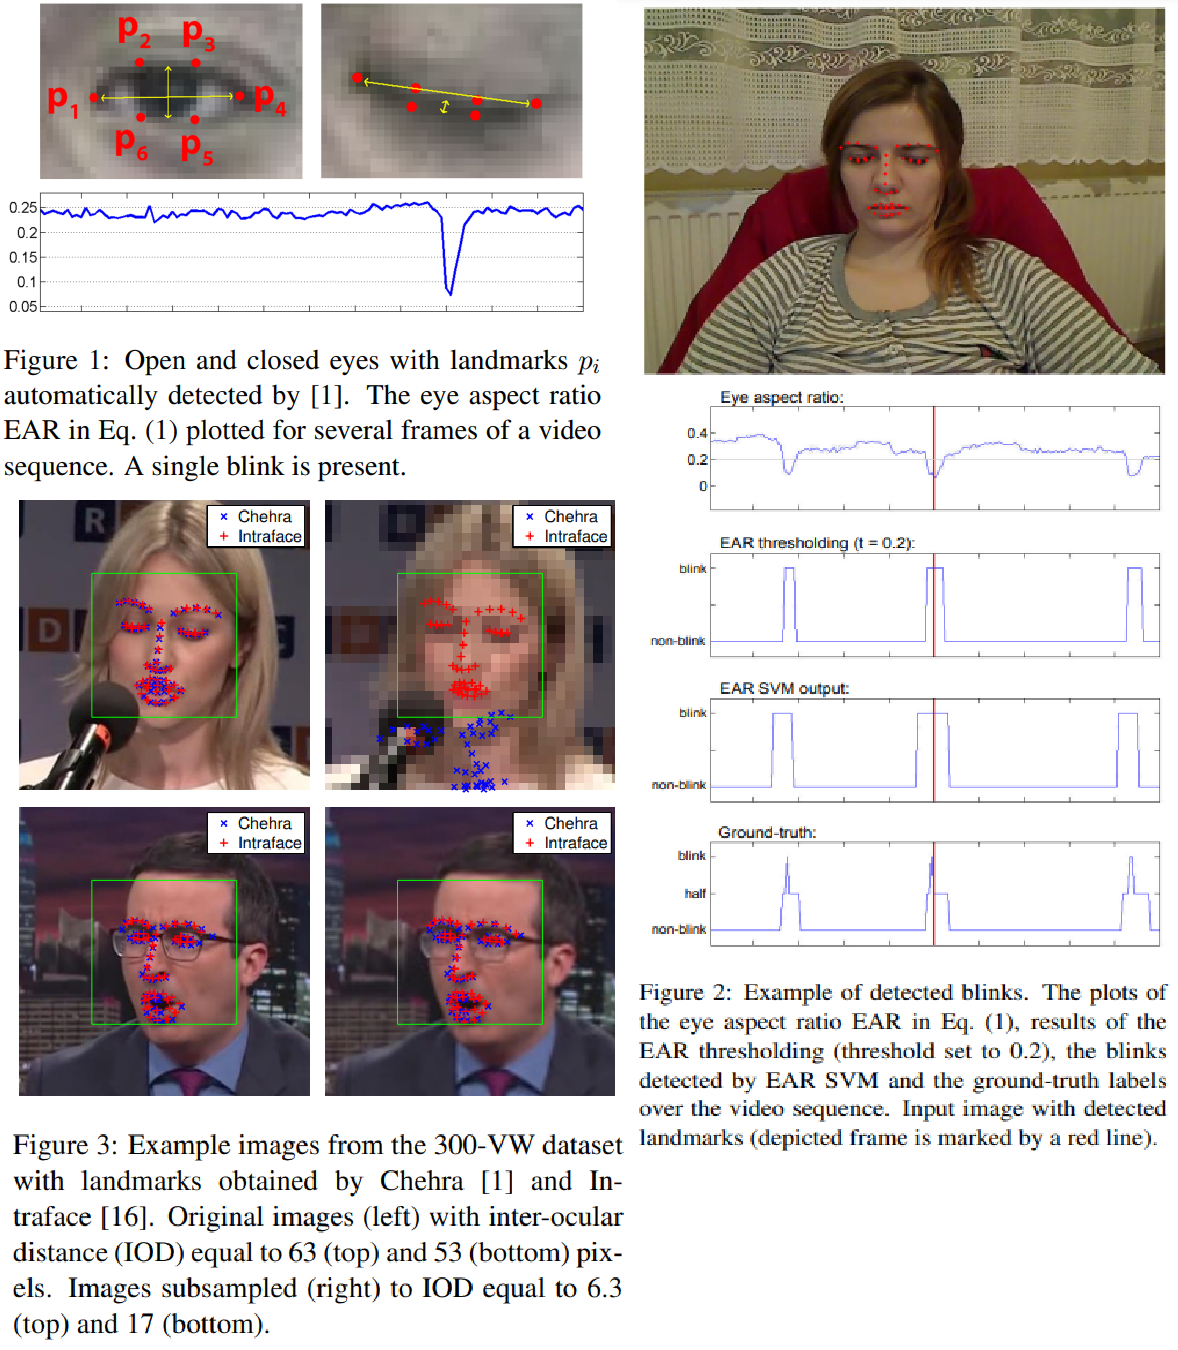
\includegraphics[width=0.80\textwidth]{img/ch3m1.png} 
\caption{实时检测标准摄像机视频序列中眨眼的算法}
\label{Test}
\end{figure}

Ching-Hua Weng 等人 \cite{weng2016driver} 提出了针对挑战赛特别会议使用 NTHU 计算机视觉实验室收集的驾驶员困倦视频数据集。整个包括训练、评估、测试的数据集包含 36 个不同种族的受试者在各种模拟驾驶场景下,所谓的场景包括正常驾驶、打哈欠、慢眨眼、入睡、爆笑记录等,而时间则在白天和夜间照明条件下都有。受试者坐在椅子上,用模拟的驱动轮和踏板玩简单的驾驶游戏时被记录下来;同时,他们在实验者的指导下进行一系列面部表情,整个数据集的总时间约为 9 个半小时。训练数据集包含 18 个主题,有 5 个 包含了 BareFace、Glasses、Night\_BareFace、Night\_Glasses、Sunglasses 的不同场景,也有每个受试者的序列,包括打哈欠和缓慢的眨眼频率,每个都记录大约 1 分钟。最后来对应于两个最重要场景的序列,嗜睡相关症状的组合如打哈欠、点头、缓慢眨眼和非嗜睡相关动作的组合如说话、大笑、看着两边,每个状态记录大约 1.5 分钟长,并评估和测试数据集包含 90 个驾驶视频(来自其他 18 名受试者),在不同场景下混合了困倦和非困倦状态。


\begin{figure}[htb]
\centering 
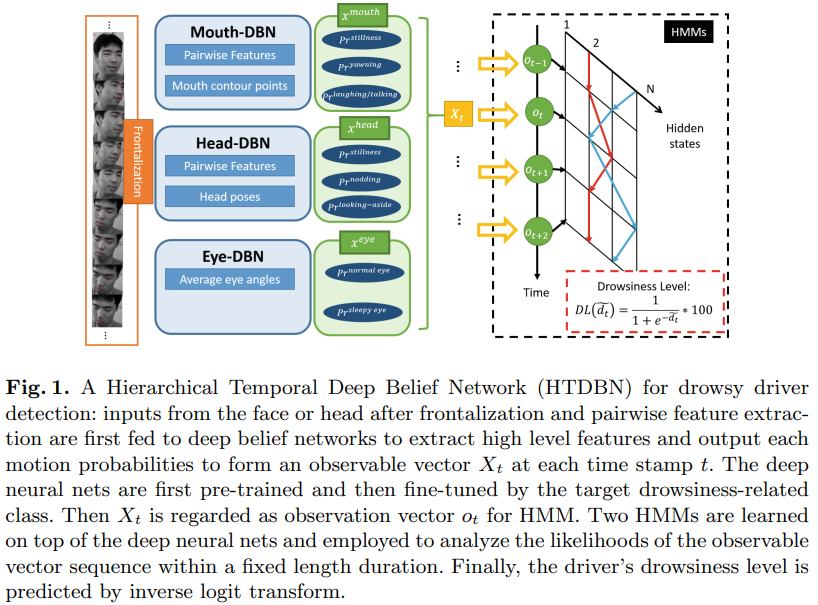
\includegraphics[width=0.80\textwidth]{img/ch3m2.png} 
\caption{A Hierarchical Temporal Deep Belief Network (HTDBN)}
\label{Test}
\end{figure}



X Luo 等人 \cite{luo2013driver} 采用不同的算法,即 AdaBoost 算法和红外帧差算法,在不同的行车光环境下定位眼睛的精确位置,研究者通过提取眼睛的特征参数来识别眼睛的状态,并基于 PERCLOS 的方法检测疲劳。同时,为了进一步测试驾驶员的疲劳程度,该研究使用局部二进制模式 (LBP) 算法来检测打哈欠作为辅助检测,其实验结果表明,该算法保证了系统的准确性,能够达到非接触式、不同光照条件和实时检测的要求。

Kaipeng Zhang 等人 \cite{zhang2016joint} 考量到由于各种姿势、照明和遮挡,在不受约束的环境中进行人脸检测和对齐上具有挑战性,而在最近的研究表明,深度学习方法可以在这两个任务上取得令人印象深刻的性能。该研究提出了一个深度级联多任务框架,利用框架它们之间的内在相关性来提高它们的性能。此外该研究框架采用级联结构,具有三个精心设计的深度卷积网络,以粗到细的方式预测人脸和地标位置。而在学习过程中,研究者提出了一种新的在线硬样本挖掘策略,可以自动提高性能,而无需手动选择样本。当中方法在具有挑战性的 FDDB 和 WIDER FACE 人脸检测基准以及用于人脸对齐的 AFLW 基准上实现了优于最先进技术的精度,同时保持了实时性能。
	\chapter{成果呈現}
\label{chap:4}

本作业根据前面等章节所归纳出来的功能需求、技术方案、理论与模型等规划,同时检索现有的开放原始码项目,对现有的部分功能进行实作,当中完成的部分概念内容如下所示,其功能分别为学习检测、作业缴交、视频观看与教学直播。

\section{学习检测}

学习检测该功能为在视频观看与教学直播的功能下,由老师方或者管理方对学生们所发起的请求,当请求的当下学生可以接受或者拒绝,并且再给定的时间中进行分析并产生统计画面。下在面的测试则是尝试针对单一功能进行分析,检测目前做到单一次,但比需等待 3 秒左右的时间落差。其实际呈现如下图所示。该功能整合基于Python PyTorch 的 YOLOv5 模型、Python Flask 后端框架与 Node.js 的 Vue 前端框架为基础,对输入的画面进行分析来辨识画面中有没有人。

\begin{figure}[htb]
\centering 
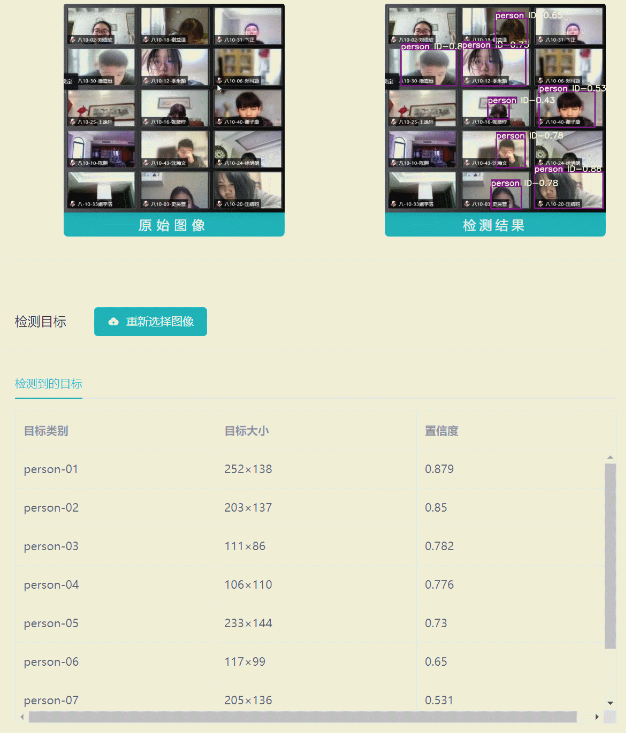
\includegraphics[width=0.80\textwidth]{img/ch4m1.png} 
\caption{学习检测}
\label{Test}
\end{figure}

\section{作业缴交}

而作业缴交的功能则是研究 Python Flask  框架的特性,研究上传档案的机制后进行尝试。困难的地方在于再要求 Python Flask 后端框架对本地伺服器资源来操作档案时,必须要额外去写设定,从测试功能中可以看到档案可以上传到指定的目录下,之后规划可以为设定档案存档于伺服器某目录下,而后台资料库存放着该档案的路径。其画面如下所示。

\begin{figure}[htb]
\centering 
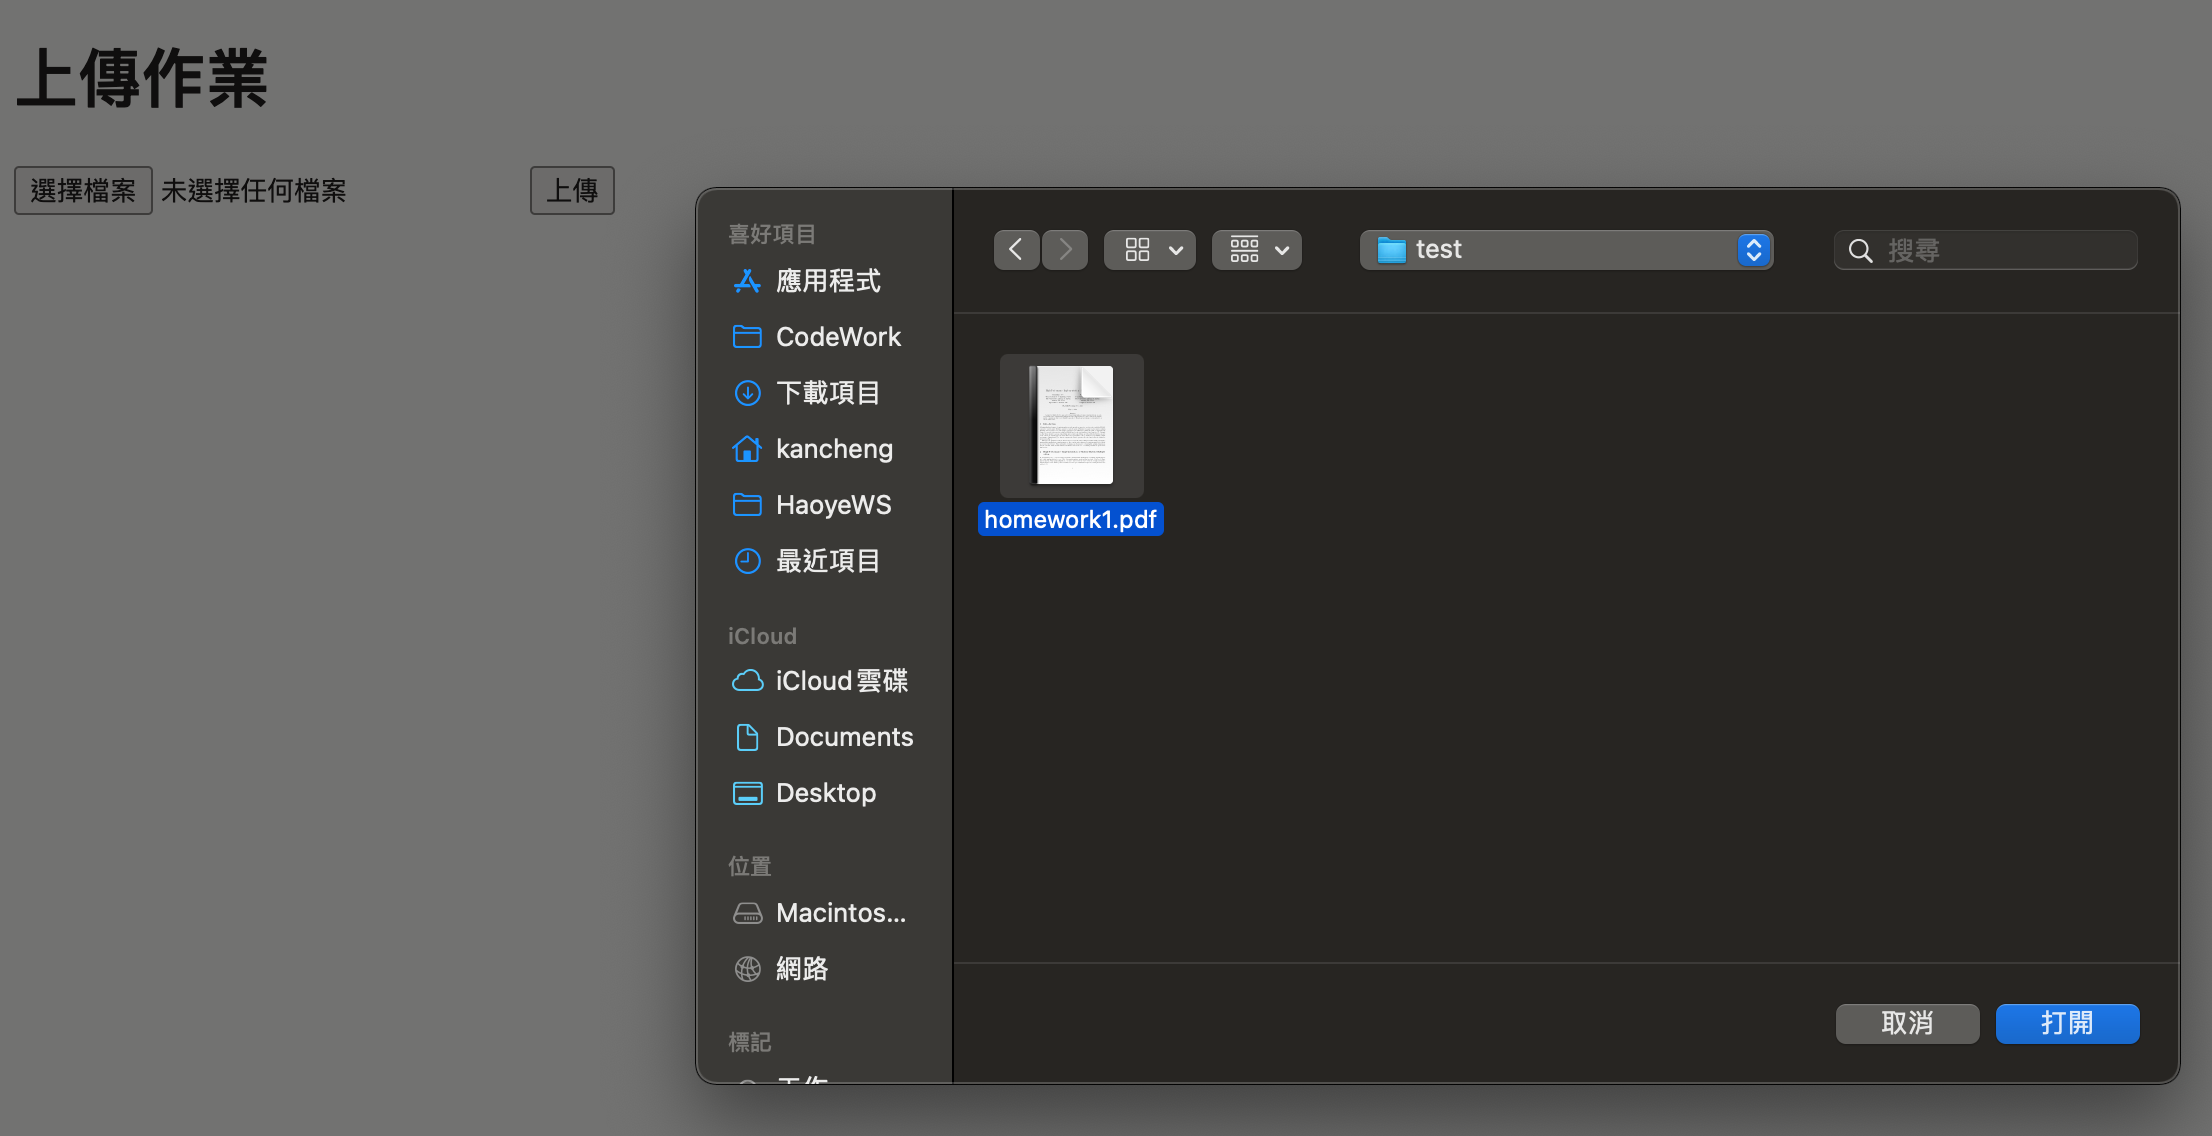
\includegraphics[width=0.80\textwidth]{img/demo-file-sys-0.png} 
\caption{作业缴交选择档案}
\label{Test}
\end{figure}

\begin{figure}[htb]
\centering 

\includegraphics[width=0.80\textwidth]{img/demo-file-sys-1.png} 
\caption{作业缴交的选择状态}
\label{Test}
\end{figure}

\section{视频观看与聊天讨论功能}

此功能则是研究 Python Flask 框架的特性,预设播放视频需要特别去设定,同时本地端汇入 JS 与 CSS 插件,则有着额外的写法,另外聊天室的部分则在此使用 Socket.io 与 Web Socket 进行处理。两部分如下所示。当中视频观看功能则可以将显示的时间进行回传。

\begin{figure}[htb]
\centering 
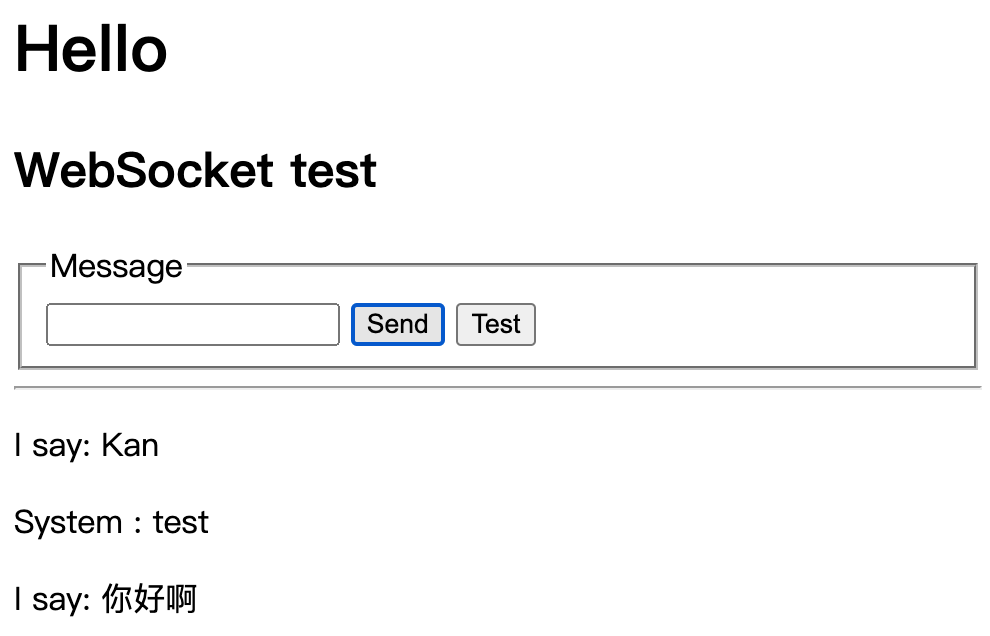
\includegraphics[width=0.80\textwidth]{img/demo-chat-sys.png} 
\caption{聊天讨论功能}
\label{Test}
\end{figure}

\begin{figure}[htb]
\centering 
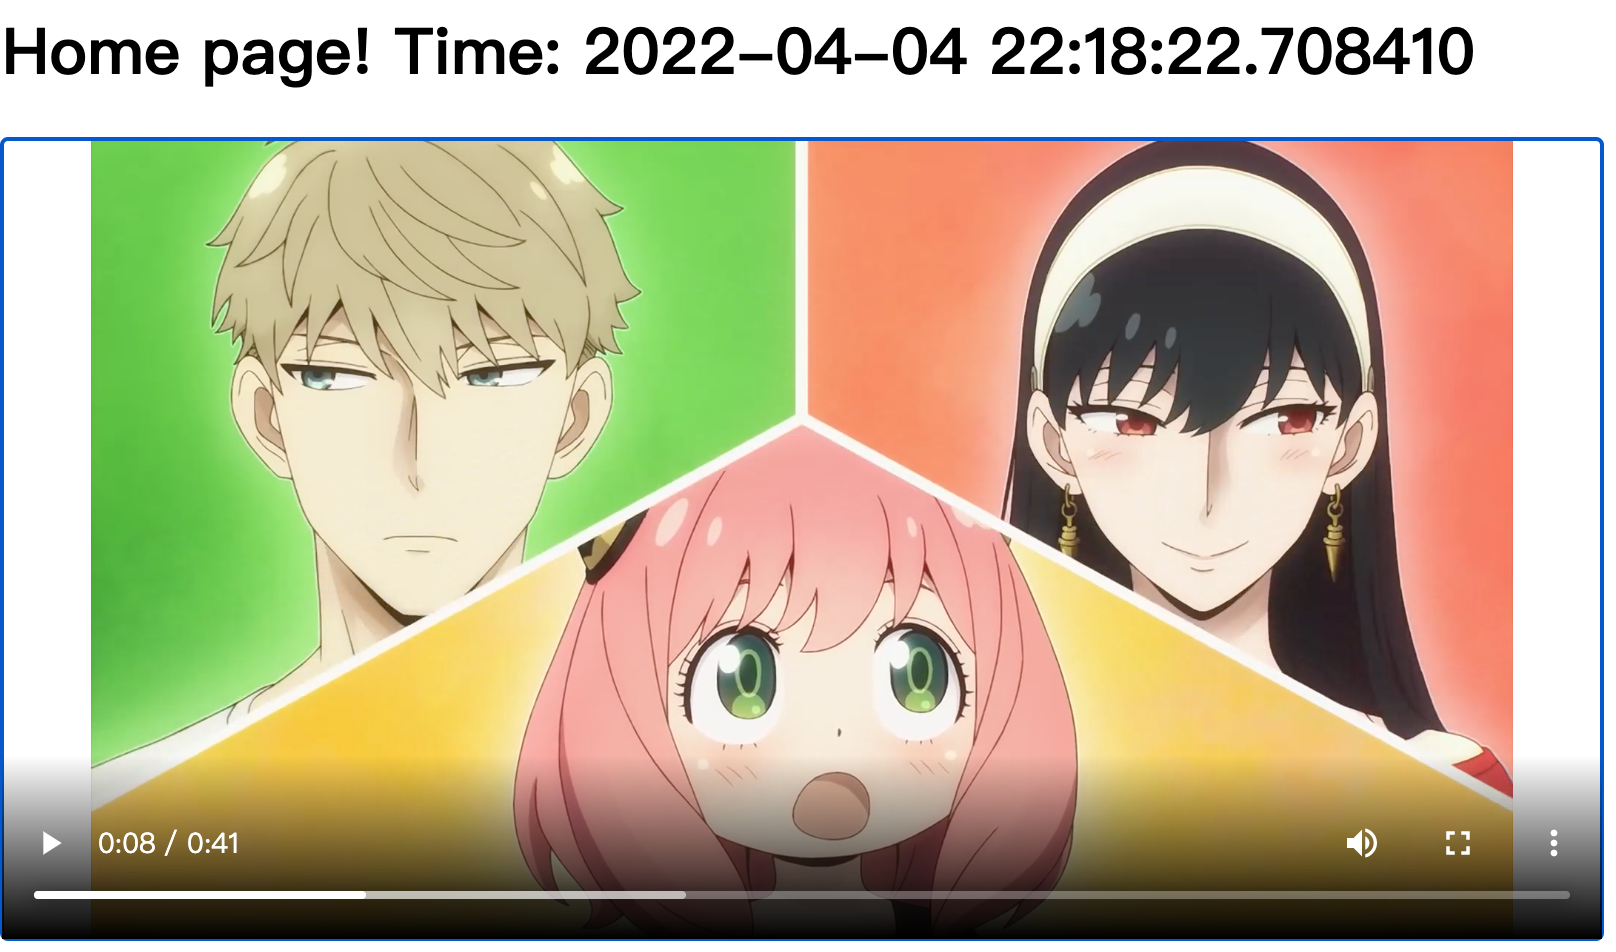
\includegraphics[width=0.80\textwidth]{img/demo-video-sys.png} 
\caption{视频观看}
\label{Test}
\end{figure}

\section{教学直播}

此功能则是研究 Python Flask 框架与 OpenCV 特性,该功能初期研究过目前的串流服务,并在本地的伺服器端考量 FFMPEG 进行处理。从测试画面中可以看到人脸辨识的画面。该测试测试功能目标在于进行串流时,辨识出人脸。未来计画与学习检测进行整合。

\begin{figure}[htb]
\centering 
\includegraphics[width=0.80\textwidth]{img/demo-streaming-sys.png} 
\caption{教学直播}
\label{Test}
\end{figure}

	\chapter{工作结论}
\label{chap:5}

本次作业从第一章对用线图绘制介面,从而确定整个系统的大致功能需求,另外从团队角度出发并考量整体成员的能力,研究所需要开发的技术跟工具,同时进行测试工作的分配。过程中讨论与分析,如何辨识学生的上课状况是否疲倦的主体原因,并找出本作业在定义流程的理论依据与文献,此作业主要贡献在于,面对深度学习与计算机视觉等研究工作下,提供一个相对稳定的 Web 服务的展示环境。同时团队也探讨整体的开发流程与技术跟研究工作的整合,因此本作业将在未来展望进行说明。

\section{未来展望}

本作业在进行开发与测试过程中讨论的三个后续发展的可用工作,分别为第一节的实际设计工具 Figma ,第二节为需要改善的团队流程,最后则是快速部属的虚拟化应用。

\subsection{实际设计}

本作业在实际用线图规划出大致的功能后,实际上要开始设计桌面应用与未来行动的使用者介面,而当中使用可以多人协作的平台 Figma,毕竟当需求厘清时,要同时考量到前端工程、测试人员、设计师广泛的讨论,当中很多功能的外观必须由此确定。

\begin{figure}[htb]
\centering 
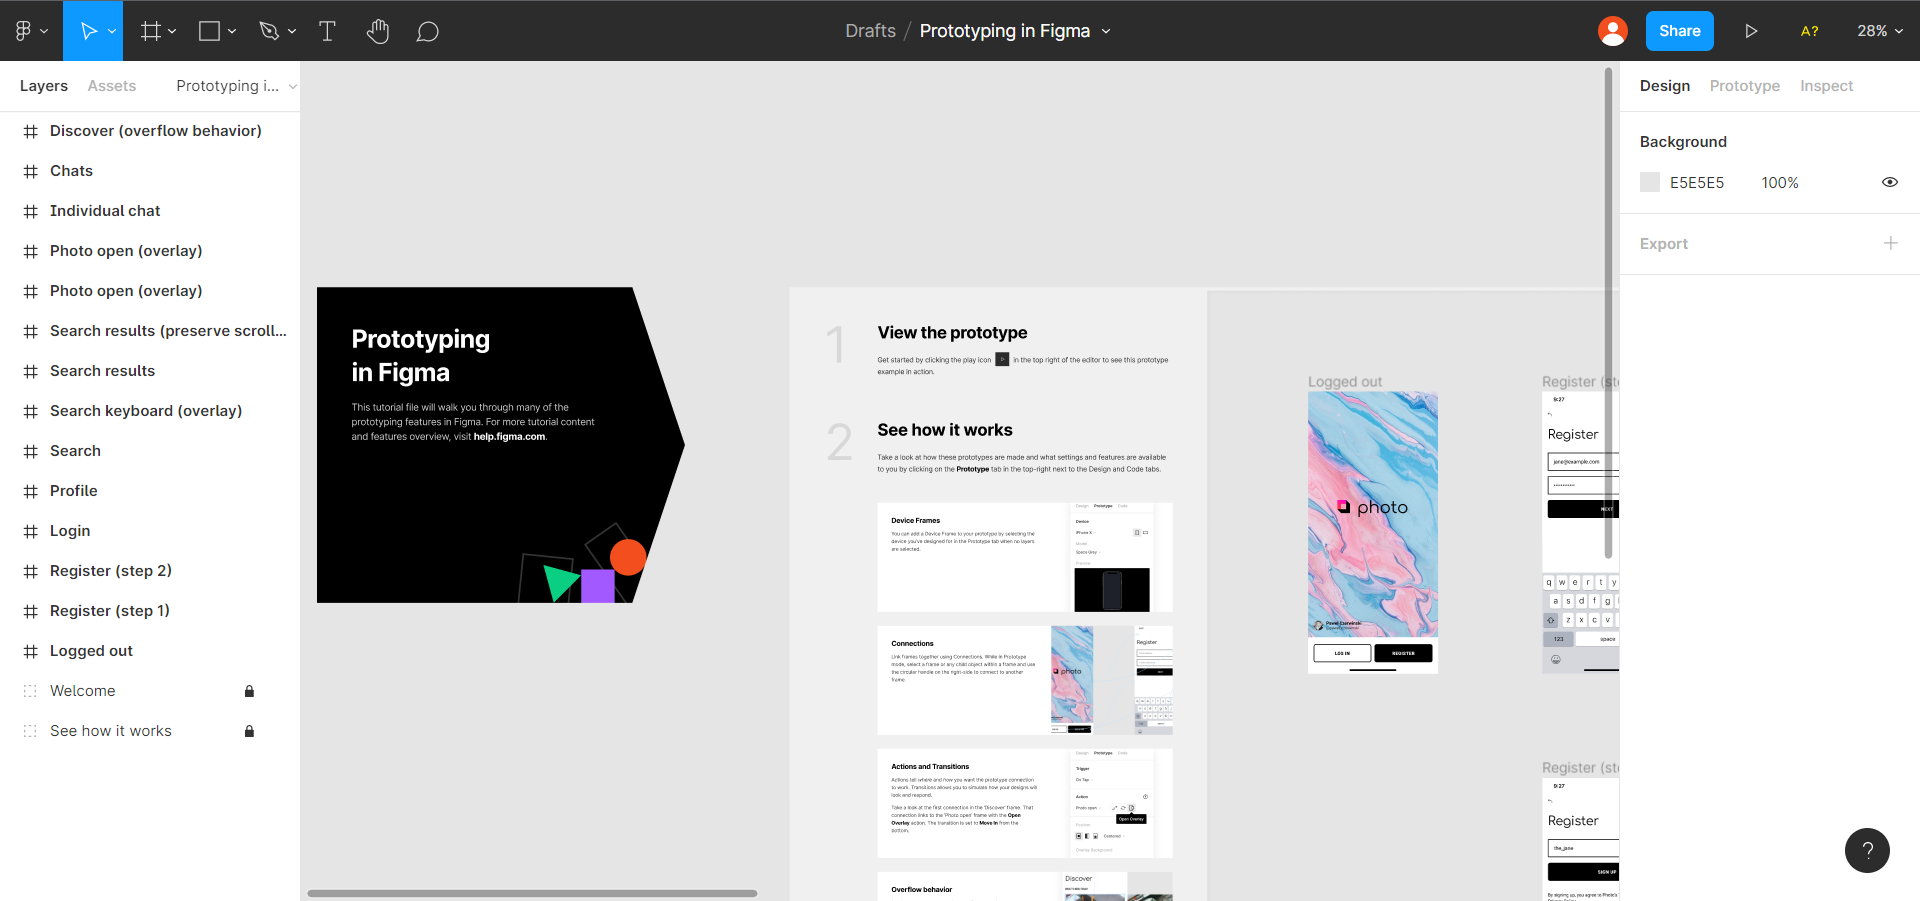
\includegraphics[width=0.80\textwidth]{img/ch5m1.png} 
\caption{Figma 平台画面}
\label{Test}
\end{figure}

\subsection{导入团队开发流程}

多人与多团队合作的状况下,不同于单人独立作业的状况,基本上在实际整个专案开发时,master 为主要的分支,一般更动会建立开发的分支, master 的更动是稳定的版本,而团队成员则是根据开发的分支 develop,再建立分支进行修正与添加新功能,完成后提出 Pull Request ,审核后合并进 develop ,其后再整合进 master ,使其系统上线。

\begin{figure}[htb]
\centering 
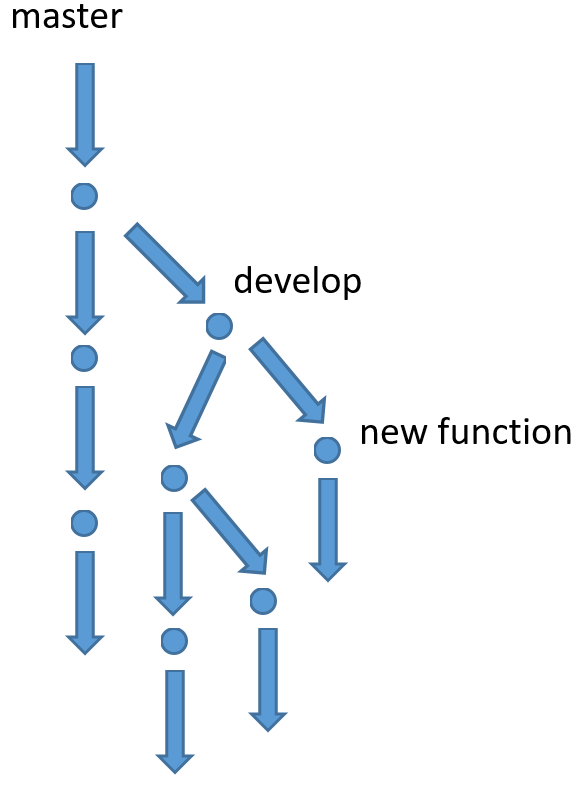
\includegraphics[width=0.80\textwidth]{img/ch5m2.png} 
\caption{Git 版本与发布概念}
\label{Test}
\end{figure}

\subsection{快速部属的工作流程}

在此主要讨论的是在持续部署与测试的考量,本次作业线上开发的过程面对大量的不同平台设备所遭遇到的环境部属问题,因此讨论 Docker 的运用,其 Docker 在开发与运维的领域中具有极大的吸引力,因为它能保持跨环境的一致性。

因为开发与发布的生命周期中,不同的环境具有细微的不同,这些差异可能是由于不同安装的版本与不同的套件和依赖关系所引起。然而 Docker 可以通过确保从开发到产品发布整个过程环境的一致性来解决这个问题。因为 Docker 容器通过相关配置,保持容器内部所有的配置和依赖关系始终不变。最终可以在开发到产品发布的整个过程中使用相同的容器来确保没有任何差异或者人工干预,加速团队的工作流程。另外以 python3.7 为基础镜像构建的 Dockerfile 编写档案如下所示。

\begin{figure}[htb]
\centering 
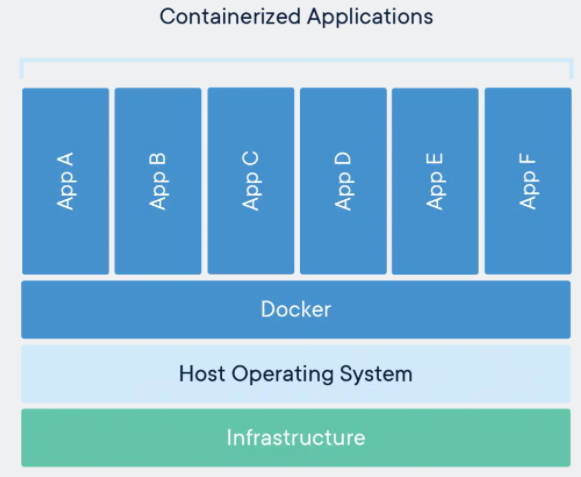
\includegraphics[width=0.80\textwidth]{img/ch5m3.png} 
\caption{Docker 概念}
\label{Test}
\end{figure}


\begin{Verbatim}
# 以 python3.7 为基础镜像构建
FROM python:3.7
# 安装nginx与supervisor
RUN apt-get update && apt-get install -y nginx supervisor
# 安装gevent与gunicorn
RUN pip install gunicorn pipenv
# 解决输出可能的中文乱码
ENV PYTHONIOENCODING=utf-8

# 创建并设置工作目录
WORKDIR /project/flask-app
# 拷贝包文件到工作目录
COPY Pipfile* /project/flask-app/
# 安装包
RUN pipenv install --system

# nginx配置相关
# 删除默认的有效配置,sites-enabled 目录下的配置文件才能够真正被用户访问
RUN rm /etc/nginx/sites-enabled/default
# 将配置文件链接到sites-available目录
RUN ln -s /etc/nginx/sites-available/nginx.conf /etc/nginx/sites-enabled/nginx.conf
# 添加自定义CMD时,添加此命令到nginx全局配置中保证容器可以跟踪到进程,防止容器退出
RUN echo "daemon off;" >> /etc/nginx/nginx.conf

# supervisord配置相关
RUN mkdir -p /var/log/supervisor
# 指定容器运行启动命令
CMD ["/bin/bash"]
\end{Verbatim}


    \appendix
    \printbibliography[heading = bibintoc]
    
    % 如有需要使用研究生成果页
    \def\cpublication{攻读硕士期间发表的论文及其他成果}

%\renewcommand{\bibname}{\cpublication}
%\begin{thebibliography}{9}{
%\zihao{5}
%\bibitem{publish} 
%\textbf{扎克·施耐德}, XXX XXX, et al. XXXX Title[C/OL]//III H D, SINGH A. Proceedings of Machine Learning Research: Proceedings of the 37th International Conference on Machine Learning: vol. 119. [S.l.]: PMLR, 2020: XXXX-XXXX. http://proceedings.ml r.press/XXXX.html.(一作,CCF-A)
%}\end{thebibliography}
%\addcontentsline{toc}{chapter}{\cpublication}


	\backmatter
	\chapter{致谢}

非常感谢 刘宏 教授,在  数字图像处理课让本次作业有机会验证目前三大主流前端框架与两种 Python 后端开发框架,并在过程中尝试将深度学习、计算机视觉与串流等主流开发方案进行调研。同时也对 Node.js、Docker、 Java 、Go 等不同方案进行测试。该工作也帮助到本作业参与同学全体,目前的开发与研究工作进度,同时也对目前深度伪造的进展有所调研,同时也将此流程在其他课程的作业上进行测试获得良好的回馈。最后感谢在这一年来一起寒窗苦读得同学与所有老师,还有默默在开源社群与前沿研究奉献的技术人员跟研究者们。
	% 需替换门户原创页pdf/扫描pdf
	%% Copyright (c) 2008-2009 solvethis
% Copyright (c) 2010-2017,2021 Casper Ti. Vector
% Copyright (c) 2021 Kurapica
% Copyright (c) 2021 iofu728
% All rights reserved.
%
% Redistribution and use in source and binary forms, with or without
% modification, are permitted provided that the following conditions are
% met:
%
% * Redistributions of source code must retain the above copyright notice,
%   this list of conditions and the following disclaimer.
% * Redistributions in binary form must reproduce the above copyright
%   notice, this list of conditions and the following disclaimer in the
%   documentation and/or other materials provided with the distribution.
% * Neither the name of Peking University nor the names of its contributors
%   may be used to endorse or promote products derived from this software
%   without specific prior written permission.
%
% THIS SOFTWARE IS PROVIDED BY THE COPYRIGHT HOLDERS AND CONTRIBUTORS "AS
% IS" AND ANY EXPRESS OR IMPLIED WARRANTIES, INCLUDING, BUT NOT LIMITED TO,
% THE IMPLIED WARRANTIES OF MERCHANTABILITY AND FITNESS FOR A PARTICULAR
% PURPOSE ARE DISCLAIMED. IN NO EVENT SHALL THE COPYRIGHT HOLDER OR
% CONTRIBUTORS BE LIABLE FOR ANY DIRECT, INDIRECT, INCIDENTAL, SPECIAL,
% EXEMPLARY, OR CONSEQUENTIAL DAMAGES (INCLUDING, BUT NOT LIMITED TO,
% PROCUREMENT OF SUBSTITUTE GOODS OR SERVICES; LOSS OF USE, DATA, OR
% PROFITS; OR BUSINESS INTERRUPTION) HOWEVER CAUSED AND ON ANY THEORY OF
% LIABILITY, WHETHER IN CONTRACT, STRICT LIABILITY, OR TORT (INCLUDING
% NEGLIGENCE OR OTHERWISE) ARISING IN ANY WAY OUT OF THE USE OF THIS
% SOFTWARE, EVEN IF ADVISED OF THE POSSIBILITY OF SUCH DAMAGE.

{
	\ctexset{section = {
		format+ = {\centering}, beforeskip = {40bp}, afterskip = {15bp}
	}}
	\specialchap{北京大学学位论文原创性声明和使用授权说明}

	% 学校书面要求本页面不要页码,但在给出的 Word 模版中又有页码。
	% 此处以学校书面要求为准。
	\thispagestyle{empty}
	
	% 替换扫描pdf,去除includegraphics前注释
	\begin{textblock}{1}(-0.8,-0.08)
		\colorbox{white}{
			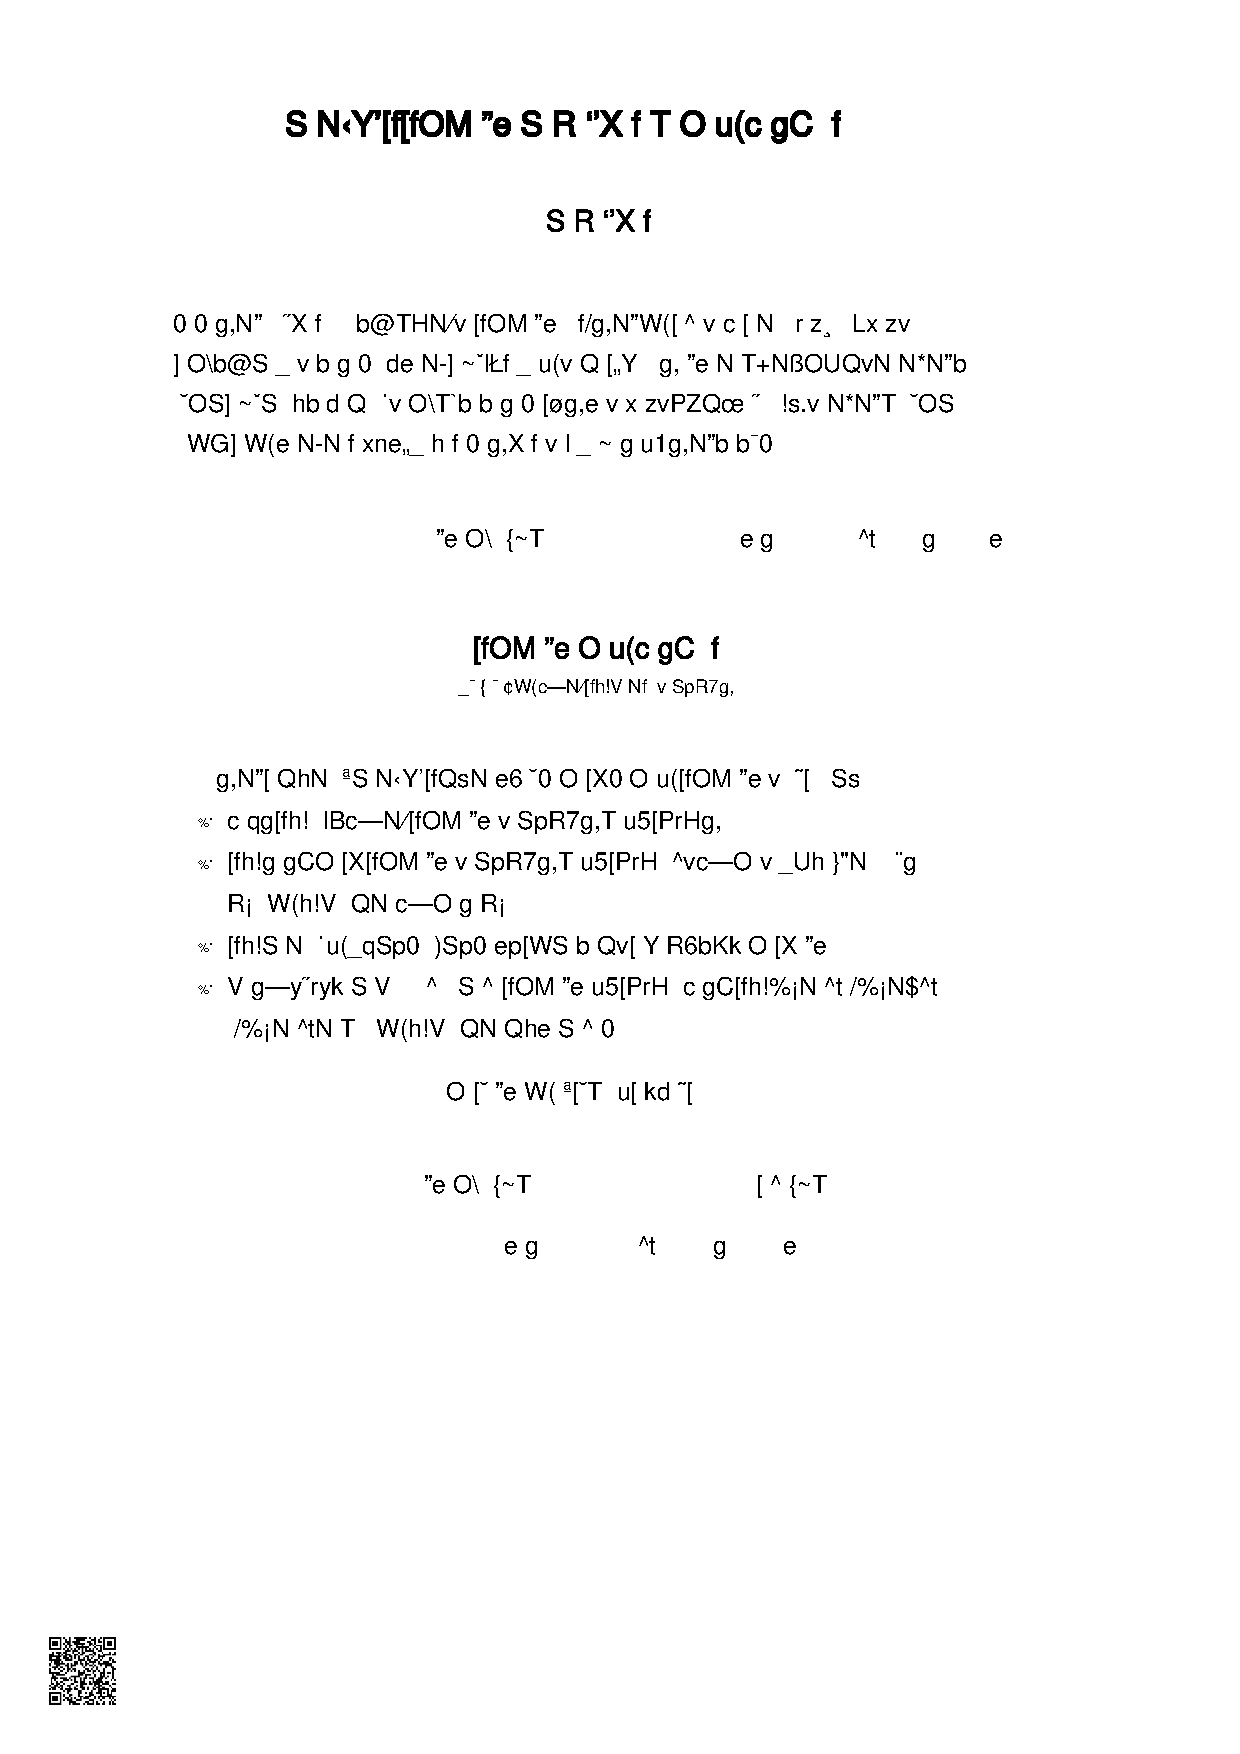
\includegraphics[height = 1.2448\textheight]{img/lwsm_180xxxxxxx.pdf}
		}
	\end{textblock}
}

% vim:ts=4:sw=4

\end{document}

% vim:ts=4:sw=4